 %美赛模板:正文部分

\documentclass[12pt]{article}  % 官方要求字号不小于 12 号,此处选择 12 号字体
% \linespread{1.1}
% \bibliographystyle{plain}
% 本模板不需要填写年份,以当前电脑时间自动生成
% 请在以下的方括号中填写队伍控制号
\usepackage[2409015]{easymcm}  % 载入 EasyMCM 模板文件
\problem{C}  % 请在此处填写题号
% \usepackage{mathptmx}  % 这是 Times 字体,中规中矩 
\usepackage{palatino}  % mathpazo 这palatino是 COMAP 官方杂志采用的更好看的 Palatino 字体,可替代以上的 mathptmx 宏包
\usepackage{pdfpages}
\usepackage{longtable}
\usepackage{tabu}
\usepackage{threeparttable}
\usepackage{listings}
\usepackage{paralist}
\graphicspath{{img/}}          % 此处{img/}为相对路径,注意加上“/”
 \let\itemize\compactitem
 \let\enditemize\endcompactitem

\newcommand{\upcite}[1]{\textsuperscript{\textsuperscript{\cite{#1}}}}
\title{M}  % 标题

% 如需要修改题头(默认为 MCM/ICM),请使用以下命令(此处修改为 MCM)
%\renewcommand{\contest}{MCM}

 %文档开始
\begin{document}

% 此处填写摘要内容
\begin{abstract}
    
 to the e s Engineering

    % 美赛论文中无需注明关键字。若您一定要使用,
    % 请将以下两行的注释号 '%' 去除,以使其生效
    \vspace{5pt}  %mm	毫米	1 mm = 2.845 pt   pt 点	1 pt = 0.351 mm
    \textbf{Keywords}:ARIMA; Fish Migration; Earnings Evaluation; Computer Simulation

\end{abstract}

\maketitle  % 生成 Summary Sheet

\tableofcontents  % 生成目录


% 正文开始
% Chapter 1: Introduction
\section{Introduction}

\subsection{Problem Background}
In today's society, tennis has evolved into one of the most visually appealing and fan-favorite sports globally. 
As of 2022, the sport has reached an impressive milestone in terms of global participation. 
There are over 100 million tennis players worldwide, encompassing all levels from amateur to professional, 
a figure that has been steadily increasing over the past decade.
Moreover, the long history of tennis is marked by many memorable matches due to their uniqueness, intensity, 
or historical significance. For instance, the 2023 Wimbledon men's singles final was a case in point. 
In this match, 20-year-old Spanish rising star Carlos Alcaraz triumphed over 36-year-old Novak Djokovic, 
thereby ending the spectacular record of one of the greatest Grand Slam players in history. 
This match was characterized by its dramatic twists and turns and continuous excitement. 
Both players experienced incredible fluctuations in performance, at times dominating the play and at others being dominated. 
This phenomenon may relate to the concept of 'momentum' experienced by a team or player in a sport. In this report, 
our team aims to use scientific and mathematical methods to measure and predict this seemingly intangible concept in the context of the match.


\subsection{Restatement of the Problem}
In this study, our team obtained data for every point played in the men's singles matches at Wimbledon 2023, 
starting from the third round onwards. 
This data acquisition was aimed at addressing the following questions:
\begin{itemize}
\setlength{\parsep}{0ex} %段落间距
\setlength{\topsep}{2ex} %列表到上下文的垂直距离
\setlength{\itemsep}{1ex} %条目间距
\item Create a model leveraging existing datasets to analyze and identify the dominating player or team at certain points in a match. 
This model should quantify their advantage and include a visualization feature. 
Moreover, the model should be customized for various sports. 
For instance, in tennis matches, 
it should reflect the server's higher likelihood of scoring. 
This approach will showcase the model's adaptability across different sports.
\item Employ the developed model to evaluate a coach's viewpoint by analyzing if the fluctuations 
in a player's 'momentum' during a match are due to random changes.
\item Based on existing data, create a new model to predict fluctuations in player performance 
during a match and identify the indicators most closely related to shifts in the game's dynamics. 
Simultaneously, use the data on past fluctuations in players' 'momentum' to provide strategies for upcoming matches between two players.
\item Conduct trials of the model across different matches and sports to assess its effectiveness in prediction and 
its applicability to sports beyond tennis. 
Following these trials, identify the model's limitations and propose additional factors that might influence its performance.
\item Compile the insights from your experiments to offer guidance about 'momentum' to tennis coaches and players. 
This will aid them in developing strategies for handling situations that affect the course of tennis matches.
\end{itemize}


\subsection{Our Work}
In athletic competitions, 'momentum' typically signifies the cumulative 'force' or 'drive' generated from various events. 
Although it's an intangible concept and challenging to measure, this task involves investigating how to quantify momentum using match data. 
We'll examine the impact of different events on momentum shifts and, using our results, 
offer targeted strategies for tennis coaches and players. Our key responsibilities include:
\begin{enumerate}[\bfseries 1.]
    \setlength{\parsep}{0ex} %段落间距
    \setlength{\topsep}{0.5pt} %列表到上下文的垂直距离
    \setlength{\itemsep}{0.5pt} %条目间距
    \item By harnessing point-by-point data from the 2023 Wimbledon men's singles (beyond the initial two rounds) and integrating it 
    with publicly accessible match statistics online, we aim to gather detailed player profiles and match data. 
    This approach will facilitate a more precise quantification and examination of momentum.
    \item Based on the existing data, develop a model that can quantitatively determine which player or team has the advantage at specific times 
    during a match. Visualize this model to assess the randomness of fluctuations throughout the course of the game.
    \item Develop a forecast model aimed at predicting variations in players' performances throughout a match, 
    pinpointing key elements that are significantly related to pivotal moments in the match.
    \item Gather and systematize match data across diverse events and sports types to evaluate 
    the predictive accuracy of the model and its applicability beyond tennis. Additionally, 
    enhance the model by including elements that were initially overlooked.
    \item Based on the model's results, provide specific advice and strategies for coaches and players in the sport of tennis.
\end{enumerate}

\section{General Assumptions}
Considering that practical problems always contain many complex factors, first of all, we need to make reasonable assumptions to simplify the model, and each hypothesis is closely followed by its corresponding explanation:

\begin{enumerate}[\bfseries \textit{Assumption} 1:]
	\item \textbf{At the beginning of a tennis match, the 'momentum' for each player or team is equally established at a value of 0.}\\
	\textbf{\textit{Explanation:}}In tennis matches, it's important to note that under certain circumstances, 
    there can be a significant difference in 'momentum' between the players before the match even begins. 
    An example is a match between someone completely unfamiliar with tennis and a world champion, 
    where their 'momentum' could differ significantly before the start. However, to simplify the model, 
    reduce the difficulty of data collection and processing, 
    our team has decided that 'momentum' in the match will only be related to the players' behavior during the game and not influenced 
    by external factors. 
    Therefore, we have set the initial 'momentum' values for both sides to be the same.
	\item \textbf{In tennis, matches played repeatedly between the same pair of players are treated as separate and independent events with no influence on each other.}\\
	\textbf{\textit{Explanation:}}The second hypothesis builds upon the first. 
    For model simplification and to ease the data collection and processing efforts, 
    our team's analysis is concentrated on the shifts in 'momentum' within the confines of 'sets', 'games', and 'points' 
    during a single tennis match. Consequently, it's established that the initial 'momentum' for both players is identical and does not vary, 
    irrespective of the number of times they have competed against each other.
	\item \textbf{The variations in 'momentum' for a particular player during a tennis match are predictable.}\\
	\textbf{\textit{Explanation:}}While a player's momentum in tennis is linked to both competitors' actions, 
    individual factors like habits, physical condition, 
    and preferences mean that a particular player's skill and tactical approach tend to remain stable across various matches. 
    Consequently, our team can use historical data on a specific player's 'momentum' fluctuations to forecast future game data changes, 
    enabling us to offer tailored recommendations before upcoming matches.
\end{enumerate}



\section{Notations}
Some important mathematical notations used in this paper are listed in Table 1. 
\begin{table}[htbp]
\begin{center}
\caption{Notations used in this paper}
\begin{tabular}{c l}
\toprule[2pt]
\multicolumn{1}{m{3cm}}{\centering Symbol}
&\multicolumn{1}{m{8cm}}{\centering Description }\\
\midrule
$x$& Longitude \\
$y$& latitude \\
$t$& The time from now \\
$u(x,y,t)$& The temperature after t years at the location with Coordinates(x, y)\\
$v(x,y,t)$& The speed after t years at the location with Coordinates(x, y) \\
$C(t)$ & The cost for fishing t years later \\
$P(t)$ & The income for fishing t years later \\
$I(t)$ & The profit for fishing t years later \\
\bottomrule[2pt]
\end{tabular}\label{tb:notation}
 \begin{tablenotes}
        \footnotesize
        \item[*] *There are some variables that are not listed here and will be discussed in detail in each section. %此处加入注释*信息
      \end{tablenotes}
\end{center}
\end{table}
\vspace{-1cm}%在\end{table}下加一行\vspace{-1cm} 其中-1的作用是缩短与下方文字距离的 切记!必须是负数


\section{Data}
\subsection{Data Collection}

\begin{table}[htbp]
\begin{center}
\caption{Data and Database Websites}
\resizebox{\textwidth}{!}
{\begin{tabular}{c c}
\toprule[2pt]
\multicolumn{1}{m{5cm}}{\centering \textbf{Database Names}}
&\multicolumn{1}{m{10cm}}{\centering \textbf{Database Websites} }\\ %m后面是列宽
\midrule
APDRC & http://apdrc.soest.hawaii.edu/ \\
NOAA & https://www.noaa.gov/ \\
HadISST & https://www.kaggle.com/carlosparadis/ \\ 
\bottomrule[2pt]
\end{tabular}}
\end{center}
\end{table}

\subsection{Data Processing}



\section{Model Preparation I}
The temperature change of ocean is determined by various factors, namely sun radia-
tion, heat loss and heat exchange of marine organisms, they can cause a significant change
of ocean temperature. Therefore, for such a complex dynamic system, a method of multiple
time series vector autoregression is applied to solve it. Formally, vector autoregression al-
gorithm can consider the spatial-temporal correlation of each variable at the same time, and
mine the data information to the maximum without introducing exogenous factors. Thus,
the prediction based on Autoregressive Integrated Moving Average model (ARIMA) is a
good approximation to the temperature field.

\subsection{Description of Temperature Field}
According to the Assumption 2, the change of ocean temperature in the vertical plane
is not considered. Therefore, for the target ocean area, based on longitude and latitude,
a coordinate system is established to describe the location of each point. Therefore, the
temperature u of any point $A \in \Omega $ at time t can be expressed as $u(x,y,t)$.

It is the coordinate of the point A, the abscissa represents the longitude and the
ordinate represents the latitude.

\subsection{Autoregressive Prediction Model}
The temperature series data of the $i$ marked fishing point in the
target sea area $i$ is numbered as 60. 
Firstly, the temperature change of each series inthe past 60 years.

It can be seen that the overall temperature variation has no obvious trend. Therefore, a
model is applied to $ARIMA(p, d, 0)$ model the temperature series data. For the $i-th$ temper-
ature series, the general situation of the model is as following
\begin{align} % 公式环境
    \Delta ^{(d)}u_{i,t} = \sum_{j=1}^{p}\alpha_{i,t}\Delta ^{(d)}u_{i,t-j} + \epsilon _{i,t}
\end{align}
Where, $\Delta ^{(d)}$ represents the difference operator of order. $\epsilon _{i,t} \sim N(0, \epsilon ^{2}_{i,t})$
is the residual value
of the model. Therefore, the first-order difference prediction value of the i-th series after the
next t years can be obtained as
\begin{align} % 公式环境
    E(\Delta ^{(d)}u_{i,t}) = \sum_{j=1}^{p}\alpha_{i,t}E(\Delta ^{(d)}u_{i,t-j})
\end{align}
Furthermore, on the basis of the assumption from ARIMA model and the practical experi-
ence, the prediction values meet the normal distribution as $u_{i,t} | u_{i,t-1} \sim N(\mu_{i,t}, \sigma^{2}_{i})$. 
Therefore, with the consideration of randomness, the initial temperature prediction formula (4) of
time t can be modified as
\begin{align} % 公式环境
    u_{i,t} = E(\Delta u_{i,t}) + u_{i,t-1} + \epsilon _{i,t}
\end{align}
Different predictions can be obtained, based on the accumulation of the randomness in the
process of progressively prediction. These relevant results which are related to the tempera-
ture change of ocean can lead the migration of fish to change. Therefore, the location of fish
can be in different areas after 50 years, which lay a great impact on the fishing companies.

\subsection{Results}
Referring to the OLS method in the linear regression model, write out the linear equa-
tions corresponding to equation as follows.That $(X^{T}X)\alpha = X^{T}Y$, 
so the closed-form solution of the corresponding parameter $ \alpha $ is
\begin{align} % 公式环境
    \alpha = (X^{T}X)^{-1}(X^{T}Y)
\end{align}
Therefore, OLS method can be used to estimate the parameters of formula. It is noted that
there are lag order and difference order in the model, so we need to perform k-fold cross
validation on the estimation results of the model, and find the model with the best prediction
effect in the given alternative models. The solution results are shown as follows,
\begin{figure}[htbp]  %h此处,t页顶,b页底,p独立一页,浮动体出现的位置
    \centering  %图表居中
    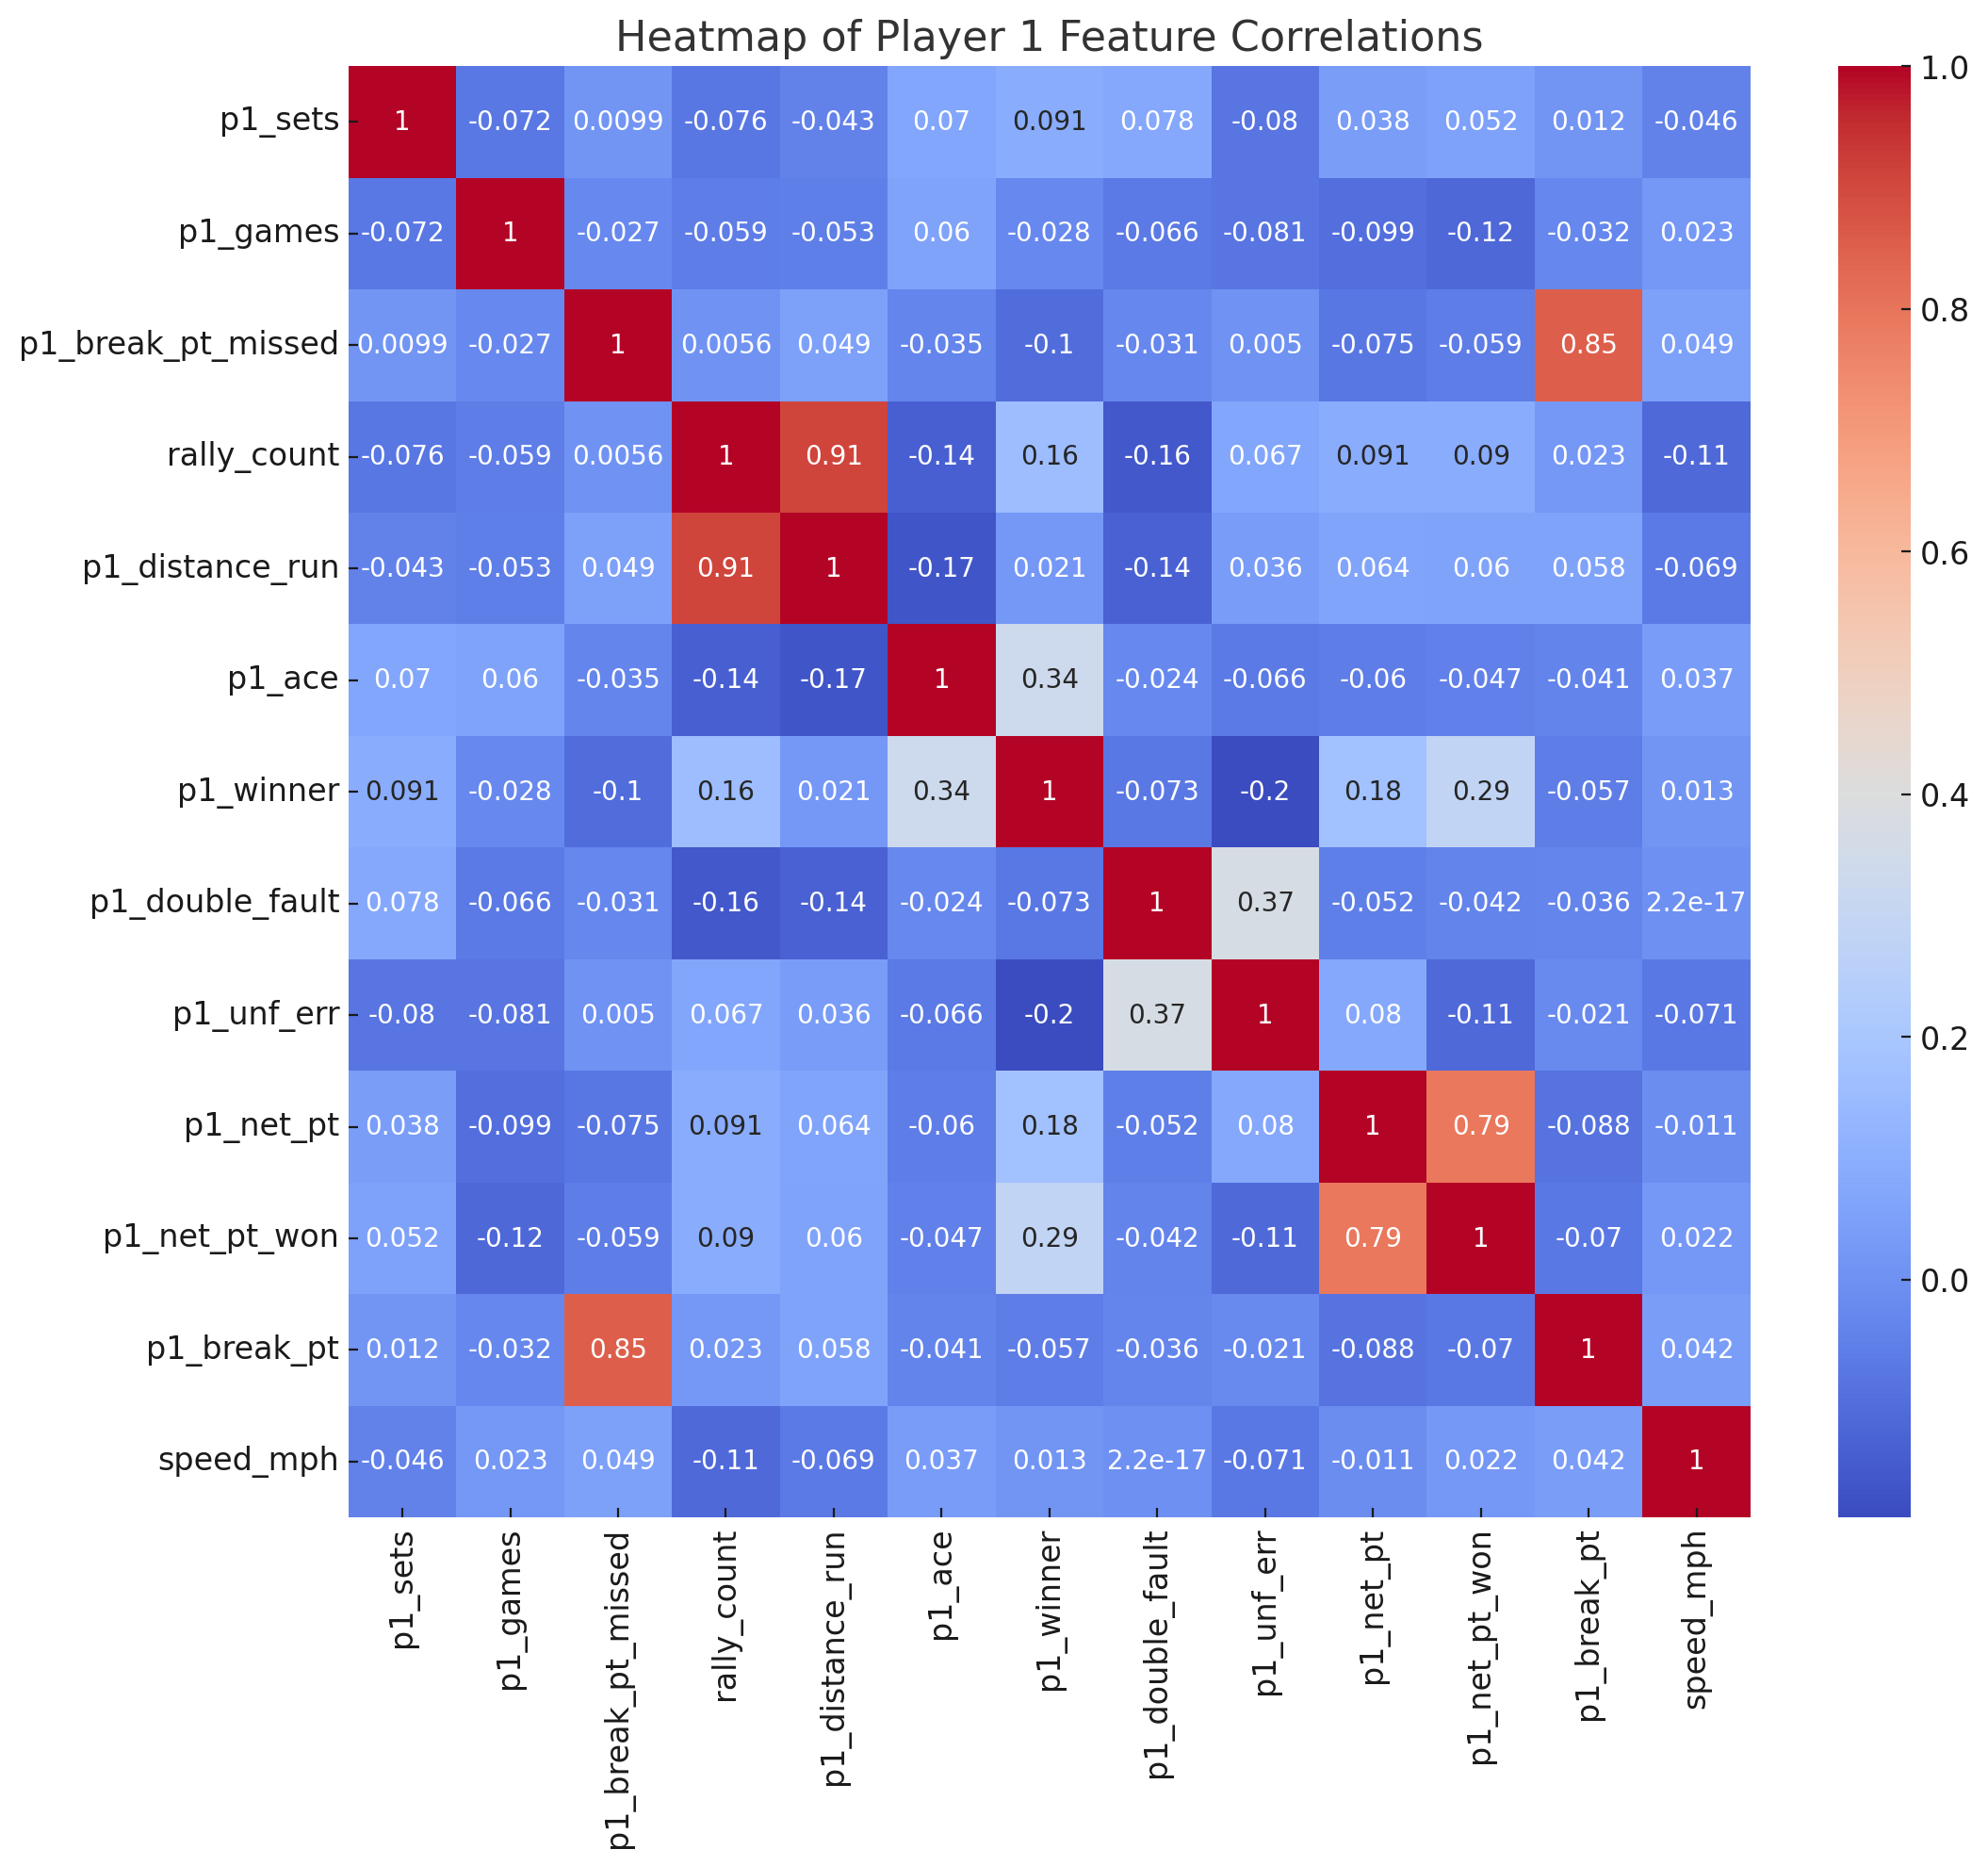
\includegraphics[width=.9\textwidth]{1.jpg} %图片的名称或者路径之中有空格会出问题 
    \caption{Choose ARIMA model by using RMSE with 6-fold cross validation} % 图片标题 
\end{figure}

It can be seen from the figure that when the lag and difference orders are both 1, the
prediction ability of the model is the best. So, we choose the optimal overall performance
ARIMA(1,1,0) model.

\section{Model Preparation II}
The migration effect of fish need to be considered from two aspects: one is to explore
the motivation and speed of fish migration based on dynamics; the other is to explore the
relationship between the position change and migration speed of fish migration based on
kinematics. A dynamic fish migration model can be obtained by combining these two as-
pects. These two parts will be described separately below.

\subsection{Kinematics of Migration}
For each point , the corresponding fish situation is shown as follows,
\begin{figure}[htbp]  %h此处,t页顶,b页底,p独立一页,浮动体出现的位置
    \centering  %图表居中
    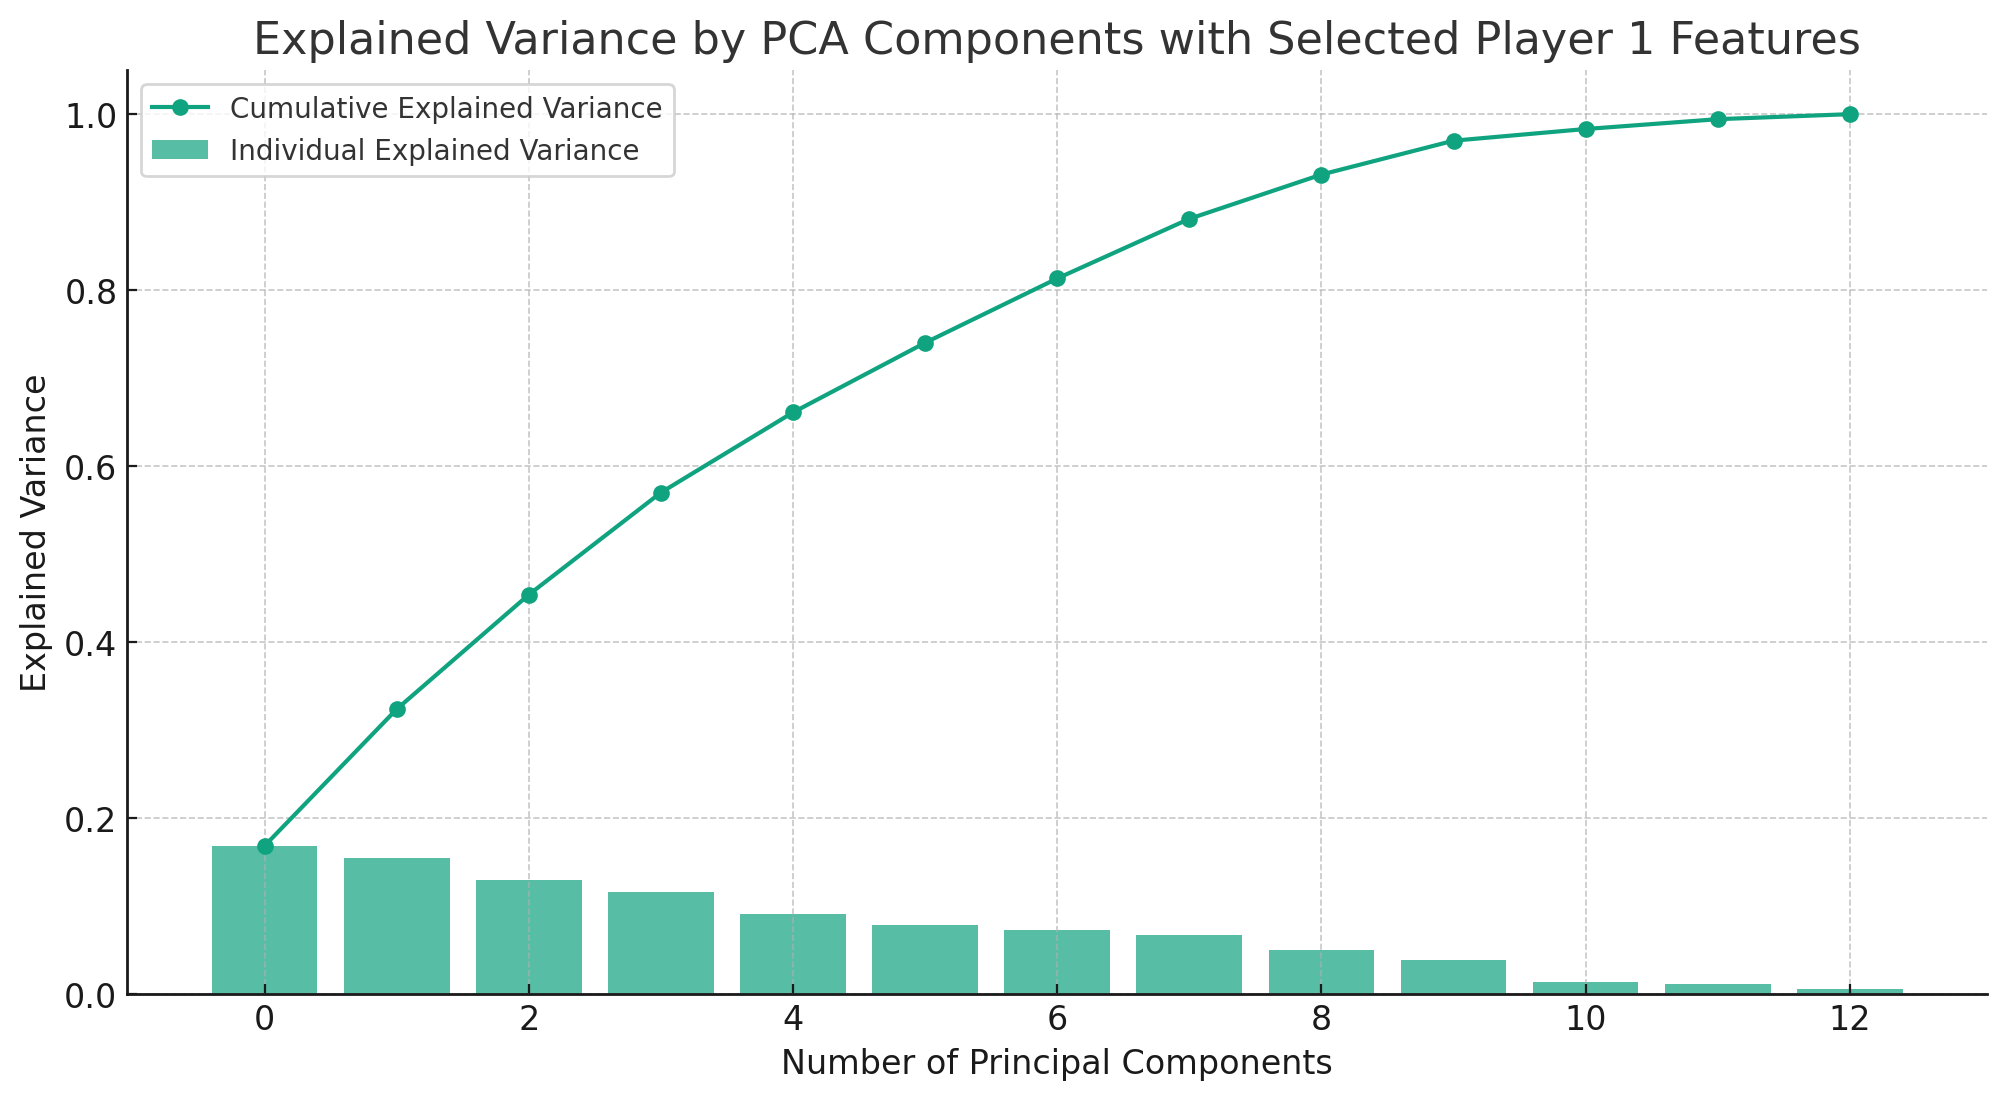
\includegraphics[width=.7\textwidth]{2.jpg} %图片的名称或者路径之中有空格会出问题 
    \caption{Fishes migration mechanism} % 图片标题 
\end{figure}

It can be seen that, for the area shown in Figure 8, the migration direction of fish is from A to B 
due to $ uA > uB > uC > uD $ . From the view of kinematics, after determining
the moving speed of fish, the position updating condition can be calculated. Therefore, the
expression of the corresponding moving speed based on the position calculation is
\begin{align} % 公式环境
    (dx, dy) = vdt
\end{align}
There, the updated formula for position (x, y) is
\begin{align} % 公式环境
    (x_{t}, y_{t}) = (x_{t-1}, y_{t-1}) + (dx, dy)
\end{align}

After the kinematic description of fish migration, it is necessary to describe and model
fish migration from the dynamic point of view. According to the living habits description of
the two kinds of fish in Section 1, the fish tend to transfer to the area with lower temperature,
so we believe that the relationship between the migration speed and the temperature field is
\begin{align} % 公式环境
    v(x,y,t) = f(\bigtriangledown u(x,,y,t))
\end{align}
Where $f()$ is an undetermined relation equation.

\subsection{Results}
According to the above formula,we have the following approximation for it.
\begin{align} % 公式环境
    \bigtriangledown u(x,y,t) = (\frac{\sigma u(x,y,t)}{\sigma x}, \frac{\sigma u(x,y,t)}{\sigma y}) 
\end{align}
Therefore, the temperature gradient at each location can be calculated by it.

According to the migration speed of Scottish herring and mackerel and the temperature
change, it is $\lim_{\Delta u \to \infty}v \to v_{max}$ and $\lim_{\Delta u \to 0}v \to 0 $. Therefore, to simplify the model, based
on the structure form of function logistic regression, the new formula can be get as follows
in the strict approximations of the equation.
\begin{align} % 公式环境
    v(x,y,t) = sign(\Delta u)\frac{\bigtriangledown u(x,y,t)}{|| \bigtriangledown u || + \beta}v_{max}
\end{align}
Based on the process of relocation, the initial distribution of fish and the distribution
after 50 years can be obtained in Figure below.
\begin{figure}[htbp]  %h此处,t页顶,b页底,p独立一页,浮动体出现的位置
    \centering  %图表居中
    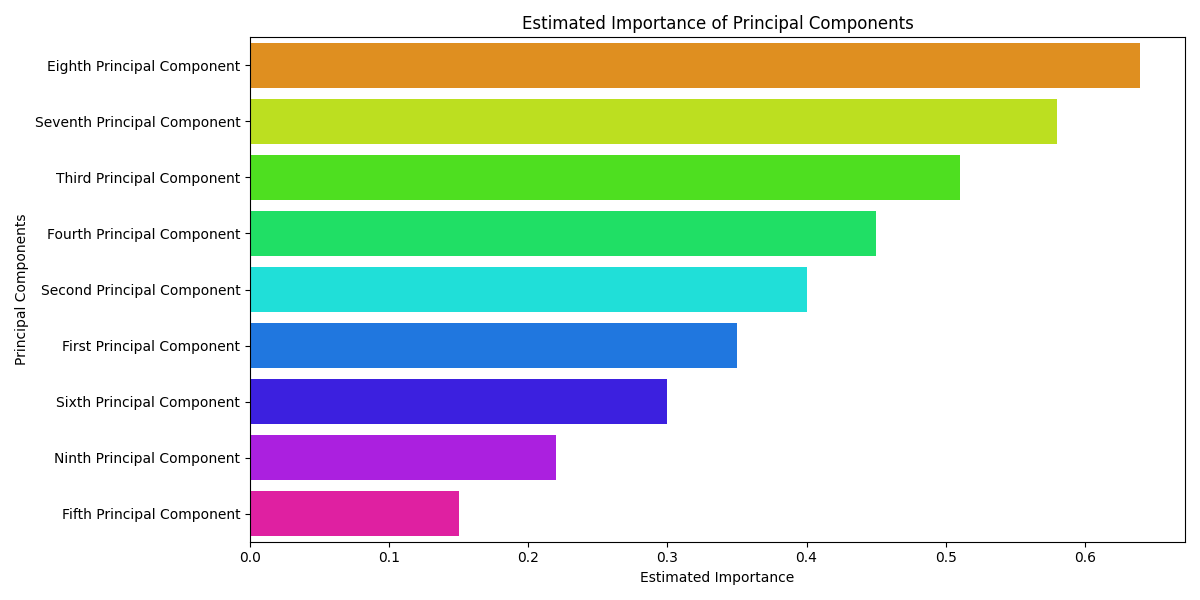
\includegraphics[width=.9\textwidth]{3.jpg} %图片的名称或者路径之中有空格会出问题 
    \caption{Prediction location of fishes over the next 50 years} % 图片标题 
\end{figure}

\section{Model Preparation III}
For the fishing companies without considering the policy factors, whether the fishing
activities can bring positive profits to the companies is the decisive factor to decide whether
they are going to sea. Therefore, it is necessary to make an effective evaluation of the cost
and benefit on fishing activities in order to determine the fishing strategy.

However, due to time constraints, in the third part of our study, which involves the predictive modeling of the operational conditions of fishing companies, our team faced a fundamental lack of theoretical grounding. Consequently, repeated attempts to develop a functional model code were unsuccessful. Therefore, this section will not be included in the report.

\section{Conclusion}
In the final analysis of this report, it must be acknowledged that due to the experimental team's inability to complete the experimental tasks in a timely manner, the objectives set for the third part of the study were not realized. Consequently, we are only able to provide the predictive outcomes for sea water temperature and fish migration patterns in the Scottish region. The analysis and conclusions regarding these two outcomes have already been discussed in their respective sections, and thus will not be reiterated here. Regrettably, from the perspective of serving as consultants for Scottish fishing companies, this experiment was unequivocally a failure. We must concede that this report fails to offer any valuable insights or recommendations for the strategic operations of fishing companies.


% 参考文献,此处以 MLA 引用格式为例
\clearpage   %另起一页继续写。这时,你最好使用“\clearpage” 
\begin{thebibliography}{99}
	\bibitem{1} HU Teng, LIU Zhanjun, LIU Yang, et al. 3D reconnaissance path planning of multiple UAVs. Journal of Systems Engineering and Electronics, 2019, 41(7): 1551-1559.
	\bibitem{2} BASBOUS B. 2D UAV path planning with radar threatening areas using simulated an-nealing algorithm for event detection. The 2018 International Conference on Artificial Intelligence and Data Processing. Malatya, Turkey: IEEE,2018: 1-7.
	\bibitem{3} WANG W F, WU Y C, ZHANG X. Research of the unit decomposing traversal method based on grid method of the mobile robot. Techniques of Automation and Applications, 2013, 32(11): 34-38.
	\bibitem{4} XU Jian, ZHOU Deyun, HUANG He. Multi UAV path planning based on improved ge-netic algorithm. Aeronautical Computing Technique, 2009, 39(4): 43-46.

\end{thebibliography}
% \includepdf[pages={1,2}]{Memo.pdf} 

\end{document}  % 结束